% ===============================================================
\section{Part 2 -- Heat-pipe heat exchanger for an electronics cabinet}
\label{sec:part2}
% ===============================================================

\subsection{Task 2.4 -- Genetic algorithm program for the heat-pipe model}
\label{sec:t24}

\paragraph{Model.}
Equation~(2.3) can be written as two thermal conductances in series:
\begin{equation}
\dot q=\frac{T_{a,in}-T_{a,out}}{\dfrac{1}{(UA)_e}+\dfrac{1}{(UA)_c\left(1+\alpha\,h_r/h_{c,ref}\right)}},\qquad
h_r=\sigma\,(T_{a,in}+T_{a,out})(T_{a,in}^2+T_{a,out}^2),
\label{eq:hp}
\end{equation}
with absolute temperatures in $h_r$, $\sigma=5.67\times10^{-8}$~W\,m$^{-2}$K$^{-4}$ and
$h_{c,ref}=80$~W\,m$^{-2}$K$^{-1}$. Over the range of the data, $h_r$ varies only between 5.8 and
7.2~W\,m$^{-2}$K$^{-1}$, i.e.\ $h_r/h_{c,ref}=0.073$--$0.090$. The radiation correction is therefore a
small, slowly varying term. As in the statement, $n_1=(UA)_e$, $n_2=(UA)_c$ and $n_3=\alpha$.

\paragraph{Program and data.}
\code{P2\_Task2.4-2.5.ipynb} is a copy of the Task~2.2 program (modifications listed in
Section~\ref{sec:codechanges}). The 122 data points of \code{CodeP2.3F26} were split at random, with a
fixed seed, into a \textbf{training set of 98 points ($80.3\,\%$)} and a \textbf{validation set of 24
points ($19.7\,\%$)}. The GA uses only the training set ($N_S=N_D=98$). The error function is the
fractional error of the heat transfer rate, Eqs.~(2.4)--(2.5). It is coded once in \code{qdot\_model()}
(Eq.~(2.6)) and used in the two locations of the code (fitness loop and population-average loop) and in the
plots. The mean absolute error (MAE) of the validation set is computed at each generation with the
population-average constants, for monitoring only.

\subsection{Task 2.5 -- Results}
\label{sec:t25}

\paragraph{Initial guesses of order one.}
Following the statement, four sets of positive initial guesses of order one were used:
Set~1 $(1,1,1)$, Set~2 $(2,2,0.5)$, Set~3 $(5,5,1)$ and Set~4 $(10,3,2)$. Each set was run with the
skeleton selection (MFRAC $=0.5$) and two mutation amplitudes ($\pm9\,\%$, $\pm30\,\%$), and with
MFRAC $=1.0$, with 3 seeds each and NGEN $=6000$ (Table~\ref{tab:t25study}).

\begin{table}[H]
\centering\scriptsize
\caption{Task 2.5: effect of the initial guesses, of the mutation amplitude and of the selection fraction
MFRAC (NGEN $=6000$, 3 seeds per line). MAE = mean absolute fractional error, Eq.~(2.5)/$N_D$. ``valid.\ MAE''
is the MAE of the validation set for the best run. ``frac.\ nkeep$=0$'' = fraction of generations without any
survivor.}
\label{tab:t25study}
\fittable{t25_study}
\end{table}

\begin{figure}[H]
\centering
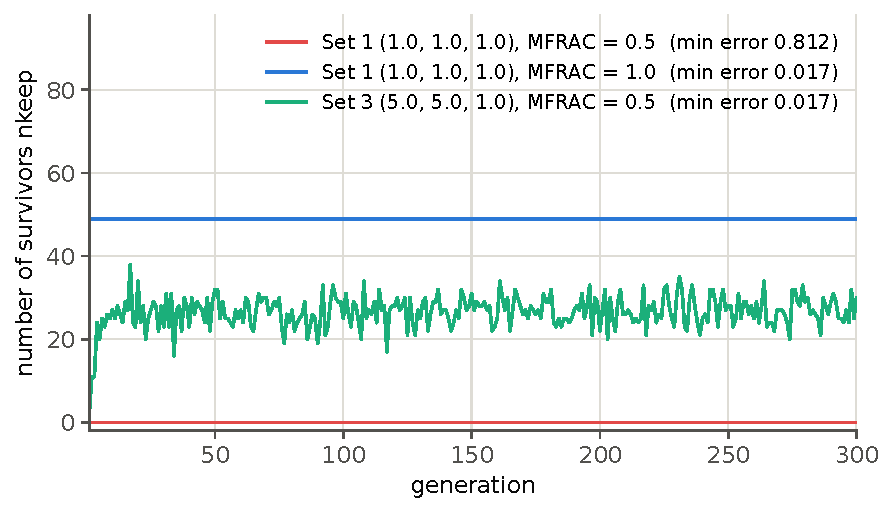
\includegraphics[width=0.66\linewidth]{figures/t25_nkeep.pdf}
\caption{Task 2.5: number of survivors per generation. With $(1,1,1)$ and the skeleton threshold
(MFRAC $=0.5$) no organism ever survives and the population is frozen. With MFRAC $=1$, half of the
population survives at every generation.}
\label{fig:t25nkeep}
\end{figure}

\begin{itemize}
  \item \textbf{Sets 3 and 4 converge immediately.} Their initial effective conductance is already
        close to the data ($\dot q/(T_{a,in}-T_{a,out})\approx2.9$~W/\textdegree C). The target 0.045 is reached in
        2--6 generations, and all runs end at a training MAE of 0.0166--0.0167.
  \item \textbf{Sets 1 and 2 do not converge at all with the skeleton algorithm, whatever the mutation
        amplitude.} The error stays at its initial value (0.81 and 0.64). Figure~\ref{fig:t25nkeep} and
        the column ``nkeep$=0$'' show why. With $(1,1,1)$, every organism predicts a heat transfer rate
        about 5 times too small, so all the fractional errors are close to $0.81$ with a very small spread.
        No error is below $0.5\times$ median, so \code{nkeep}$\,=0$ at \emph{every} generation. The
        offspring are then all mutations of organism \code{n[0]}, and this organism is never replaced
        (offspring are stored from index \code{nkeep+1}). Each generation is a new random cloud around the
        same frozen parent, nothing accumulates, and a larger mutation amplitude does not help.
  \item \textbf{With MFRAC $=1$} (the organisms with an error below the median survive), half of the
        population survives at every generation. Sets 1 and 2 then converge (target reached after 84 and 55
        generations) to the same error as Sets 3 and 4. Changing a single selection parameter turns a
        frozen algorithm into a robust one.
\end{itemize}

\paragraph{Effect of the number of generations.}
Table~\ref{tab:t25ngen} shows that, once the population is in the right region, NGEN has almost no effect.
From $(5,5,1)$, 100 generations already give the final error. From $(1,1,1)$ with MFRAC $=1$, about
500--2000 generations are needed. More generations do not lower the validation error either (no
over-fitting with only 3 constants): once converged, it stays between 0.0204 and 0.0208.

\begin{table}[H]
\centering\small
\caption{Task 2.5: effect of NGEN (range over 3 seeds; MUT $=\pm9\,\%$).}
\label{tab:t25ngen}
\fittable{t25_ngen}
\end{table}

\paragraph{Best fit.}
The best run (lowest \emph{training} error; the validation set was not used to select it) is
\TwoFiveBestSet\ $(5,5,1)$ with NGEN $=\TwoFiveBestNgen$ (seed \TwoFiveBestSeed):
\begin{center}
\begin{tabular}{@{}l c@{}}
\toprule
$n_1=(UA)_e$ & \TwoFiveNone~W/\textdegree C\\
$n_2=(UA)_c$ & \TwoFiveNtwo~W/\textdegree C\\
$n_3=\alpha$ & \TwoFiveNthree\\
\midrule
MAE, training set (98 points) & \textbf{\TwoFiveFtrain}\\
MAE, validation set (24 points) & \textbf{\TwoFiveFval}\\
MAE, all 122 points & \TwoFiveFall\\
overall conductance $UA_{eff}=[1/n_1+1/(n_2(1+n_3\bar h_r/h_{c,ref}))]^{-1}$ & \TwoFiveUA~W/\textdegree C\\
\bottomrule
\end{tabular}
\end{center}
Both errors are \textbf{far below the 0.045 target}: training $\TwoFiveFtrain$, validation $\TwoFiveFval$.
The deterministic check gives the same training minimum ($\TwoFiveRefF$). The validation MAE is slightly
higher than the training MAE, as expected for points that were not used in the fit. Figure~\ref{fig:t25evol}
shows the evolution of the run, Figure~\ref{fig:t25parity} the predicted versus data heat transfer rates
(training points as circles, validation points as squares), and Figure~\ref{fig:t25surf} the surface
$\dot q(T_{a,in},T_{a,out})$ over the range of the data. The largest deviations are at the smallest heat
transfer rates (e.g.\ 8.6~W for a temperature difference of only 3.4\,\textdegree C). There, a temperature uncertainty
of $\pm0.1$\,\textdegree C already gives $\pm3\,\%$ on the driving temperature difference.

\begin{figure}[H]
\centering
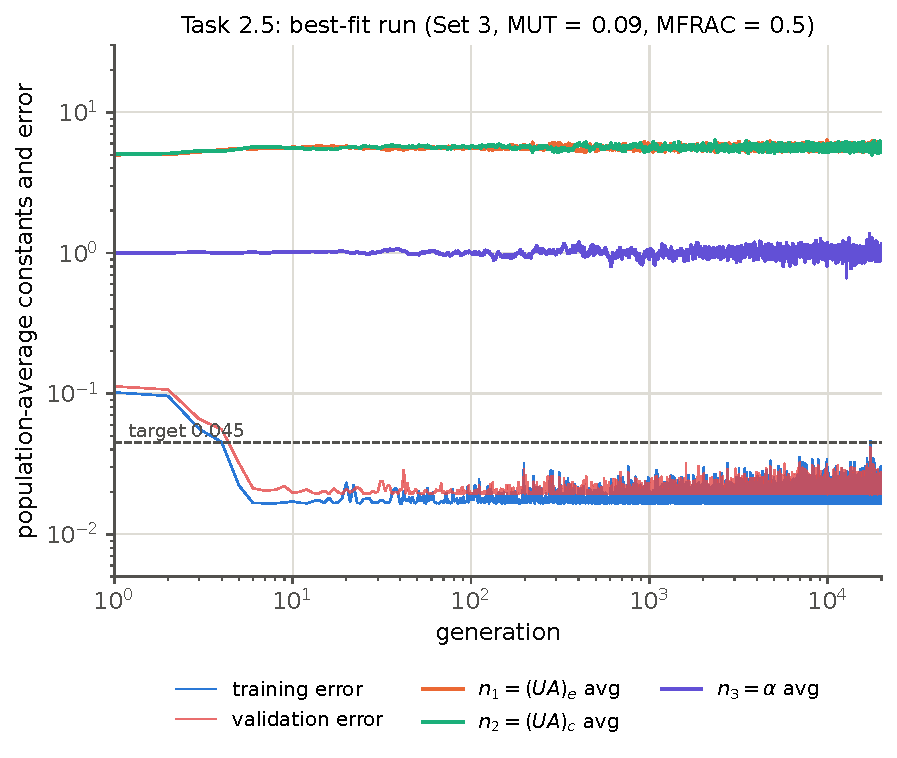
\includegraphics[width=0.7\linewidth]{figures/t25_evolution.pdf}
\caption{Task 2.5: evolution of the training and validation errors and of the population-average
constants for the best-fit run.}
\label{fig:t25evol}
\end{figure}

\begin{figure}[H]
\centering
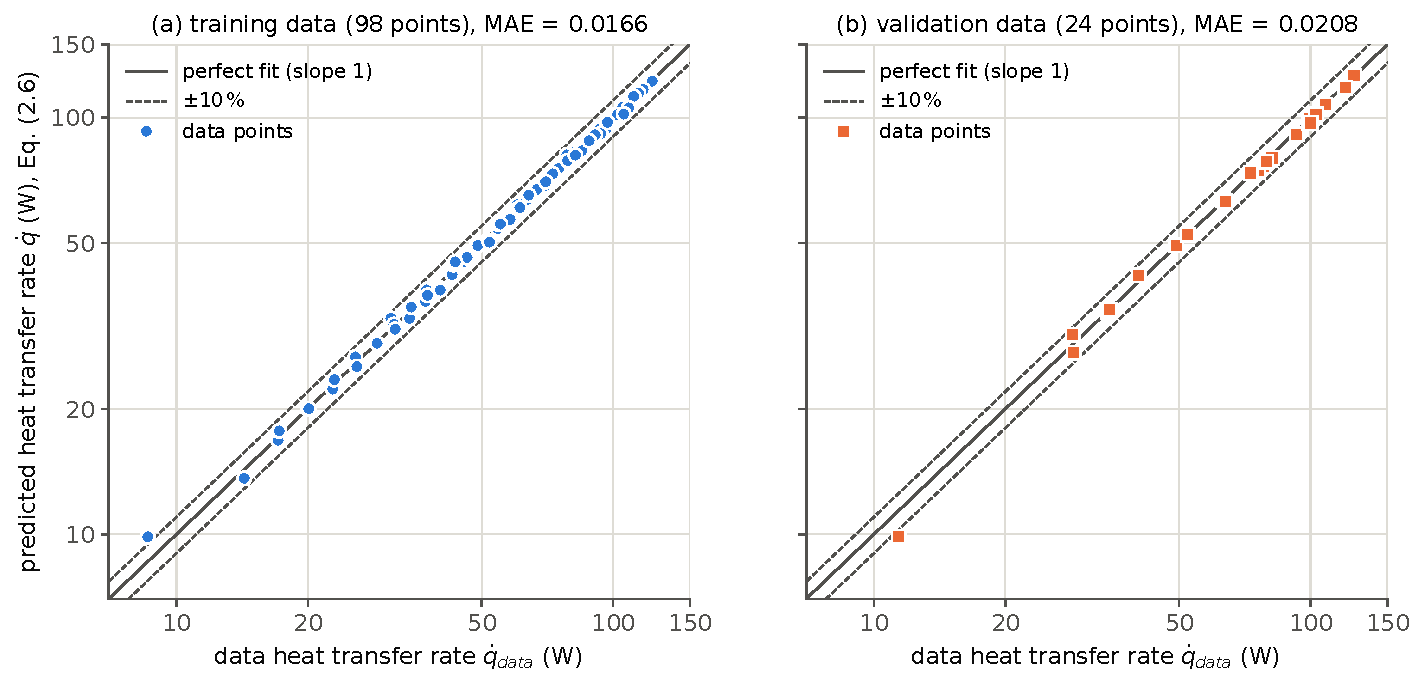
\includegraphics[width=\linewidth]{figures/t25_parity.pdf}
\caption{Task 2.5: predicted versus data heat transfer rate (log-log) for (a) the training data (circles)
and (b) the validation data (squares).}
\label{fig:t25parity}
\end{figure}

\begin{figure}[H]
\centering
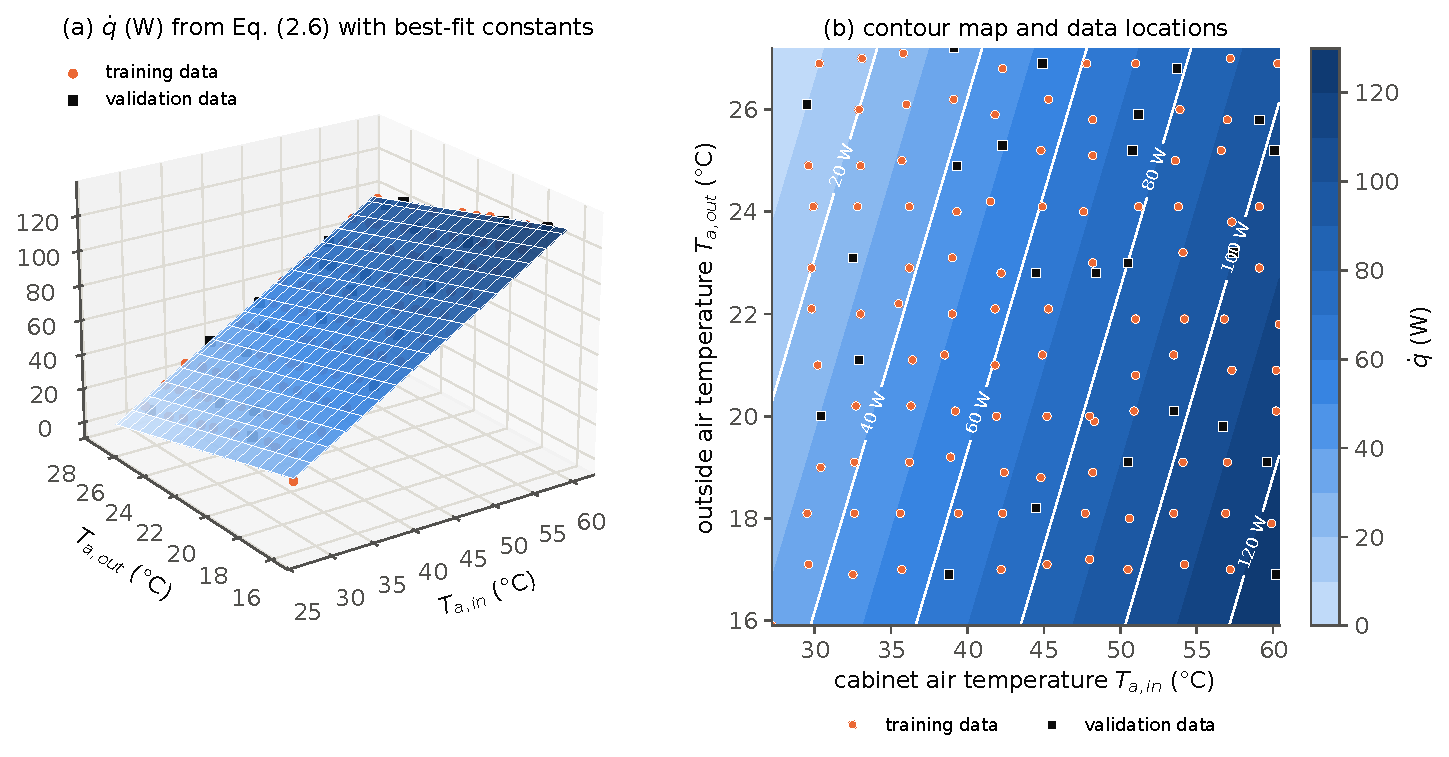
\includegraphics[width=\linewidth]{figures/t25_surface.pdf}
\caption{Task 2.5: heat transfer rate predicted by Eq.~(2.6) with the best-fit constants as a function of
$T_{a,in}$ and $T_{a,out}$ over the range of the data: (a) surface with the data points; (b) contour map.}
\label{fig:t25surf}
\end{figure}

\paragraph{How unique are $(UA)_e$, $(UA)_c$ and $\alpha$?}
Table~\ref{tab:t25study} shows that runs with the same error give quite different constants.
Figure~\ref{fig:t25deg} explains this. When $(UA)_e$ is fixed anywhere between 3.2 and 1000~W/\textdegree C and the
two other constants are re-optimised, the training MAE changes only from $\TwoFiveProfMinF$ to
$\TwoFiveProfMaxF$. The $\TwoFiveNconv$ converged GA runs give $(UA)_e=\TwoFiveConvNoneMin$--$\TwoFiveConvNoneMax$,
$(UA)_c=\TwoFiveConvNtwoMin$--$\TwoFiveConvNtwoMax$ and $\alpha=\TwoFiveConvNthreeMin$--$\TwoFiveConvNthreeMax$,
but the series conductance $UA_{eff}$ only varies between $\TwoFiveConvUAMin$ and $\TwoFiveConvUAMax$~W/\textdegree C
($\pm0.3\,\%$). The data contain only the overall conductance $UA_{eff}$ (two resistances in series)
and its weak temperature dependence through $h_r$. \textbf{They cannot separate the evaporator and
condenser conductances.} The final constants are therefore set by the initial guesses: the GA stops at the
point of the valley closest to where it started. Starting from equal guesses $(UA)_e=(UA)_c$, as for Set 3,
it returns nearly equal values ($5.7$ and $5.4$~W/\textdegree C). This is physically sensible, because the evaporator
and condenser fin sections of Fig.~2.1 have the same length (0.25~m). It also gives $\alpha\approx1.1$, so
radiation increases the condenser conductance by about $9\,\%$. To determine $(UA)_e$ and $(UA)_c$
separately, an additional measurement would be needed, e.g.\ the heat-pipe wall (vapour) temperature.

\begin{figure}[H]
\centering
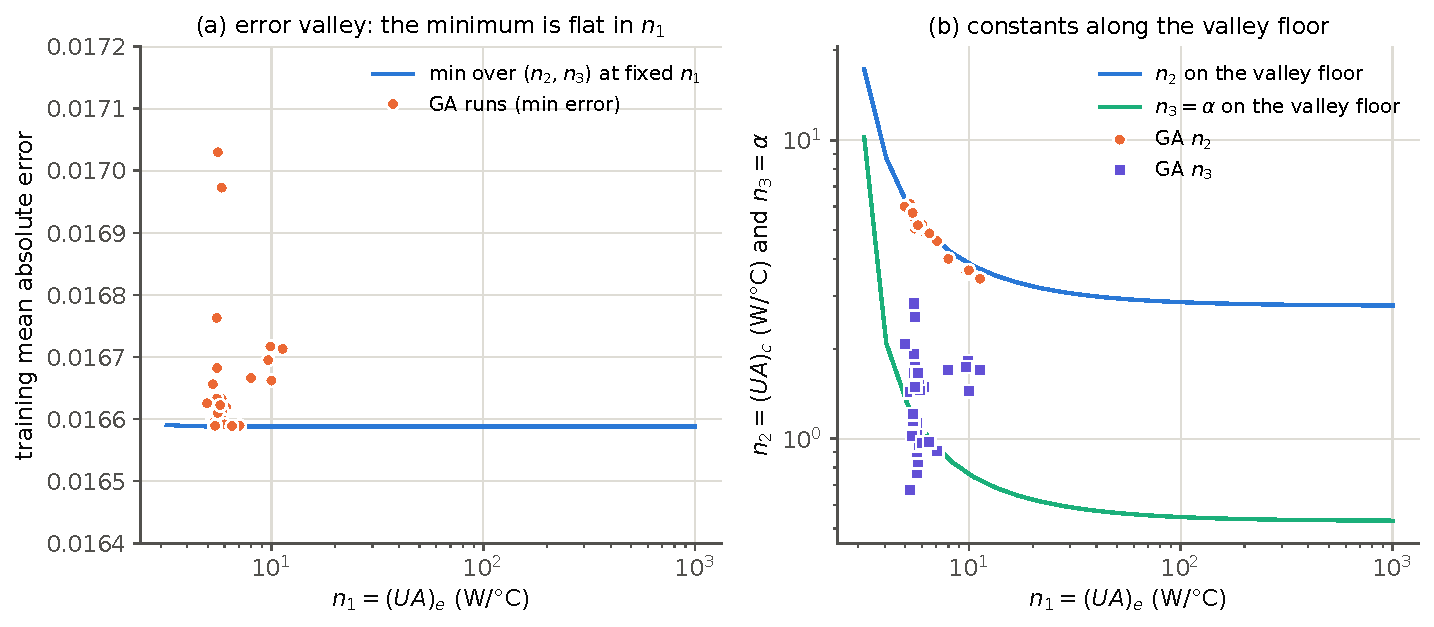
\includegraphics[width=\linewidth]{figures/t25_degeneracy.pdf}
\caption{Task 2.5: (a) minimum training error when $(UA)_e$ is fixed and $(UA)_c$, $\alpha$ are
re-optimised, with the converged GA runs; (b) values of $(UA)_c$ and $\alpha$ along the bottom of the
valley.}
\label{fig:t25deg}
\end{figure}
